\documentclass[]{article}
\usepackage{amsmath}
\usepackage{amsthm}
\usepackage{listings}
\usepackage[margin=1.3cm]{geometry}
\usepackage{graphicx}
\usepackage{hyperref}
%\usepackage{cleveref} %for the cref command

\title{Practical Lab Numerical Computing Computational Finance \\Bachelor-Worksheet 3}
\author{Lukas Troska, Ilja Kalmykov}
\date{}
\setlength{\parindent}{0pt}

\begin{document}

\maketitle

The source code can be found at \url{https://github.com/iljaGH/CompFin/}.

\section*{Task 2}
Implementation of closed form solution for discrete and continuous geometric average Asian option. See task2.cpp for code.

\section*{Task 3}
Convergence of discrete geometric average option with $S(0)=10,r=0.1,\sigma=0.25,T=1,K=10$ for both $M=10$ and $M=200$ time steps against closed-form solution.
As we can see, the number of time steps does not affect the convergence.
\begin{figure}[!ht]
\centering
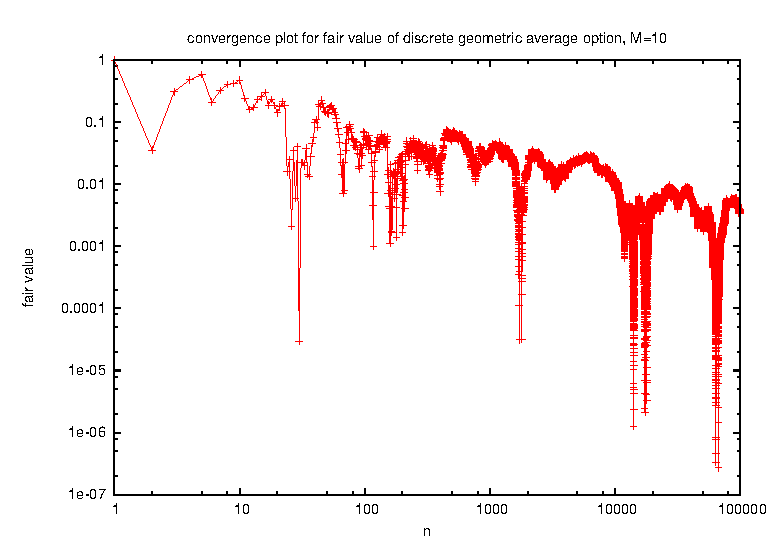
\includegraphics[width=.9\textwidth]{task3_10.eps}
\caption{Convergence plot for the fair value of discrete geometric average
option, $M = 10$}
\label{fig:Task3a}
\end{figure}
\begin{figure}[!ht]
\centering
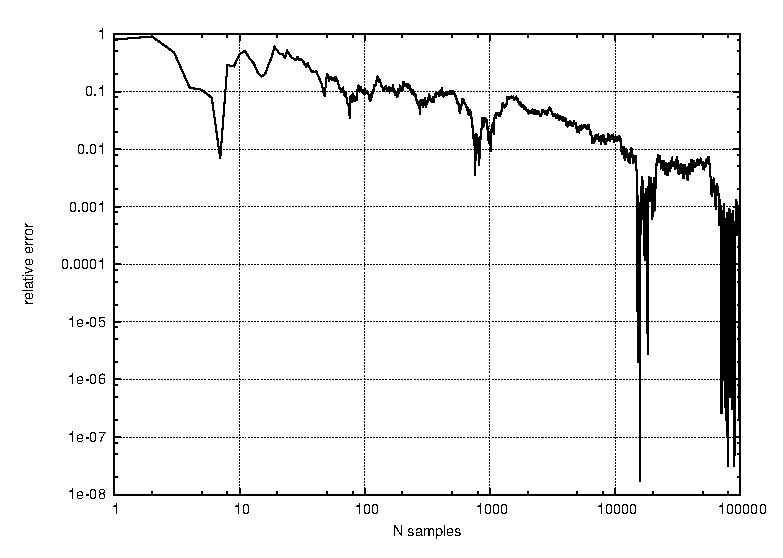
\includegraphics[width=.9\textwidth]{task3_200.eps}
\caption{Convergence plot for the fair value of discrete geometric average
option, $M = 200$}
\label{fig:Task3b}
\end{figure}
\clearpage

\section*{Task 4} Approximation of continuous geometric average option by discrete geometric average option with $S(0)=10,r=0.1,\\\sigma=0.25,T=1,K=10$. See task4.cpp for code.
\begin{figure}[!ht]
\centering
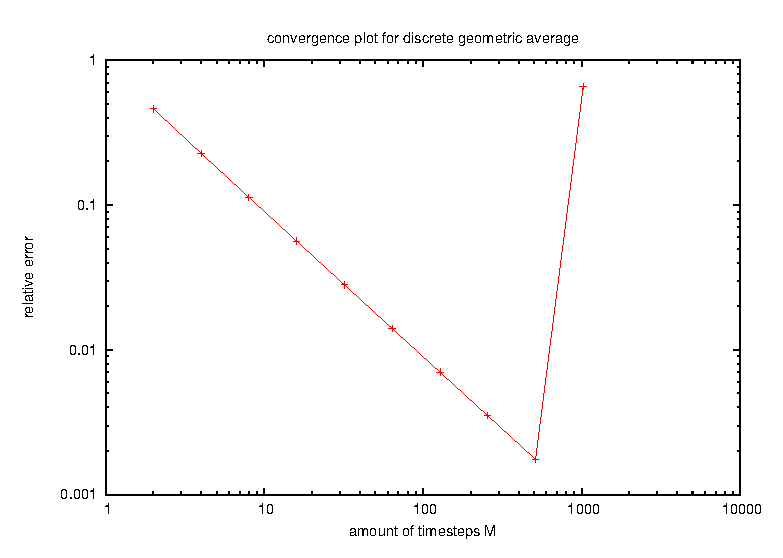
\includegraphics[width=.9\textwidth]{task4.eps}
\caption{Convergence plot for the discrete geometric average option}
\label{fig:Task4}
\end{figure}
\clearpage

\section*{Task 5} Integrand of the discrete arithmetic average for $M=2,S(0)=10,r=0.1,\sigma=0.25,T=1,K=10$. See task5.cpp for code.\\
\begin{figure}[!ht]
\centering
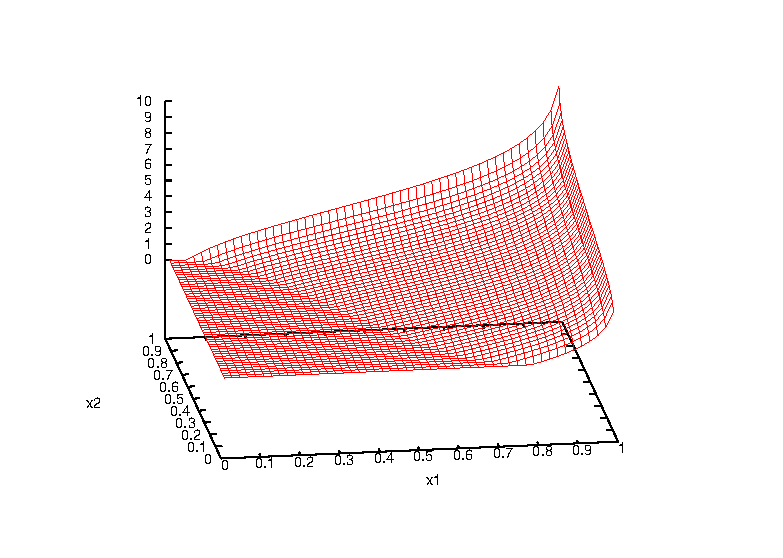
\includegraphics[width=.9\textwidth]{task5_1}
\caption{Integrand of discrete arithmetic average}
\label{fig:Task5}
\end{figure}

\section*{Task 6}
Implementation of Halton sequence. See task6.cpp for code.
\clearpage

\section*{Task 7} The first plot is a plot of the
first 100 members of the Halton sequence for $d=2$ and 100 uniform random numbers on
$(0,1)^2$ in the second plot. As we can see, the Halton sequence covers the
unit square more evenly than uniformly distributed points, i.e. "gaps" between the points are not as
big. See task7.cpp for code. \\
\begin{figure}[!ht]
\centering
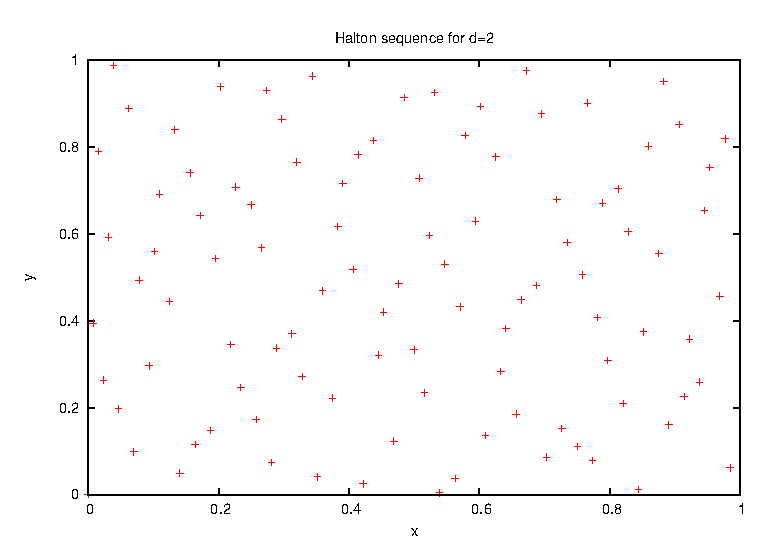
\includegraphics[width=.9\textwidth]{task7_halton.eps}
\caption{Halton sequence (2-dimensional, first 100 members)}
\label{fig:Task7a}
\end{figure}
\begin{figure}[!ht]
\centering
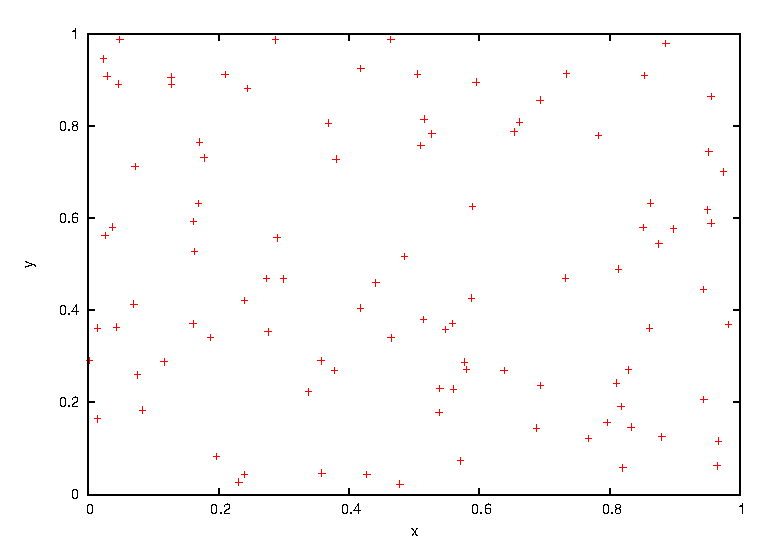
\includegraphics[width=.9\textwidth]{task7_uniform.eps}
\caption{100 uniform random numbers on $(0,1)^2$}
\label{fig:Task7b}
\end{figure}
\clearpage




\section*{Task 8}
Implementation of d-fold tensor product for given univariate quadrature formula. See task8.cpp for code.

\section*{Task 9}
Nodes of different product grids.\\
\begin{figure}[!ht]
\centering
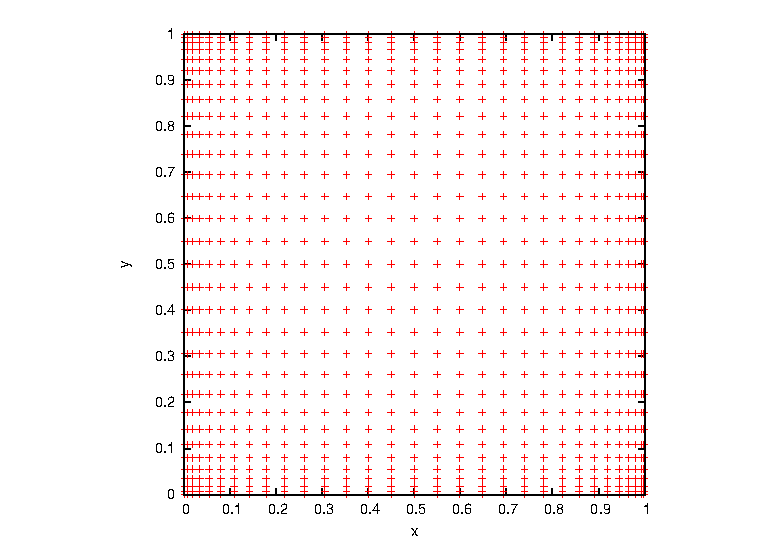
\includegraphics[width=.9\textwidth]{task9_gauss}
\caption{Gauss-Legendre product grid at level 5}
\label{fig:Task9a}
\end{figure}

\begin{figure}[!ht]
\centering
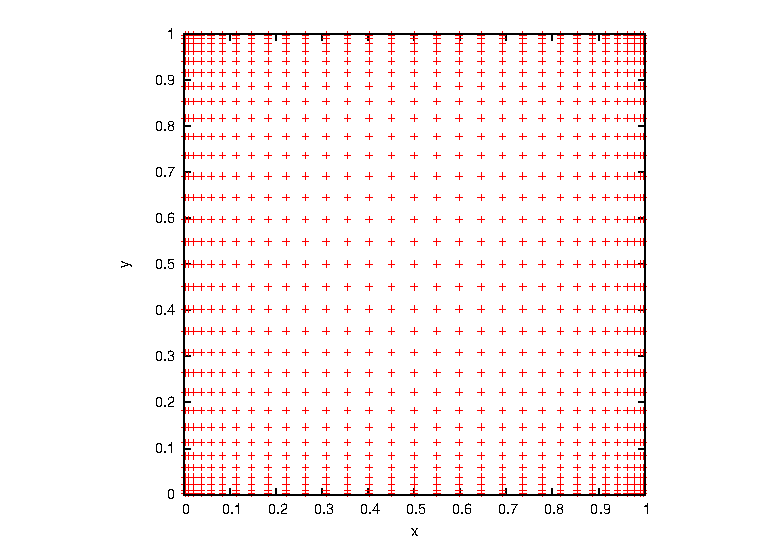
\includegraphics[width=.9\textwidth]{task9_cc}
\caption{Clenshaw-Curtis product grid at level 5}
\label{fig:Task9b}
\end{figure}

\begin{figure}[!ht]
\centering
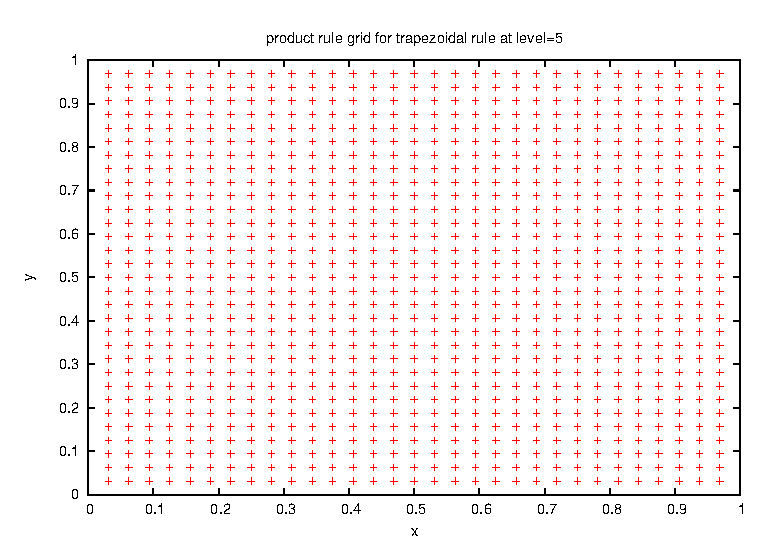
\includegraphics[width=.9\textwidth]{task9_trapezoidal}
\caption{Trapezoidal product grid at level 5}
\label{fig:Task9c}
\end{figure}
\clearpage

\section*{Task 10}
Implementation of sparse grid quadrature method. See task10.cpp for code.

\section*{Task 11}
Nodes of different sparse grids.\\
\begin{figure}[!ht]
\centering
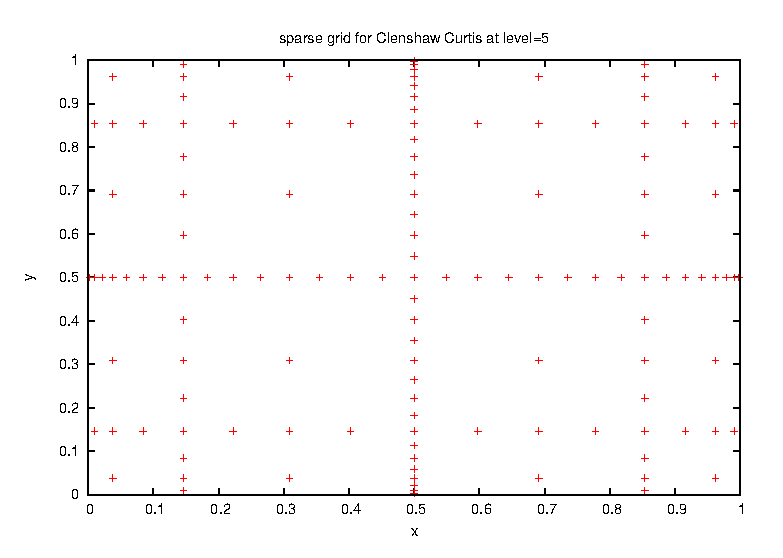
\includegraphics[width=.9\textwidth]{task11_cc5}
\caption{Clenshaw-Curtis sparse grid at level 5}
\label{fig:Task11a}
\end{figure}

\begin{figure}[!ht]
\centering
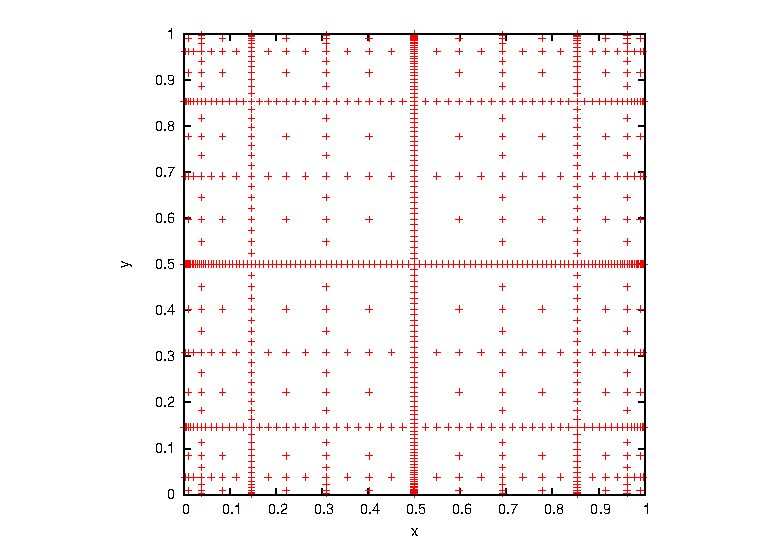
\includegraphics[width=.9\textwidth]{task11_cc7}
\caption{Clenshaw-Curtis sparse grid at level 7}
\label{fig:Task11b}
\end{figure}

\begin{figure}[!ht]
\centering
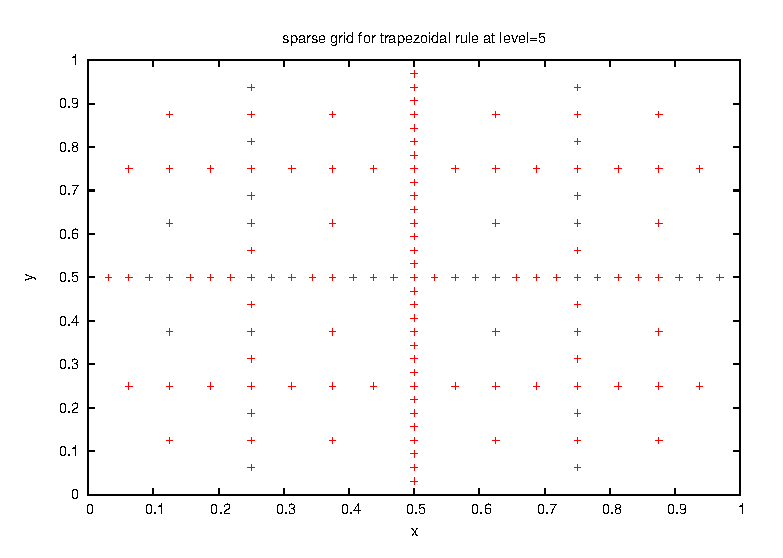
\includegraphics[width=.9\textwidth]{task11_trap_5}
\caption{Trapezoidal sparse grid at level 5}
\label{fig:Task11c}
\end{figure}

\begin{figure}[!ht]
\centering
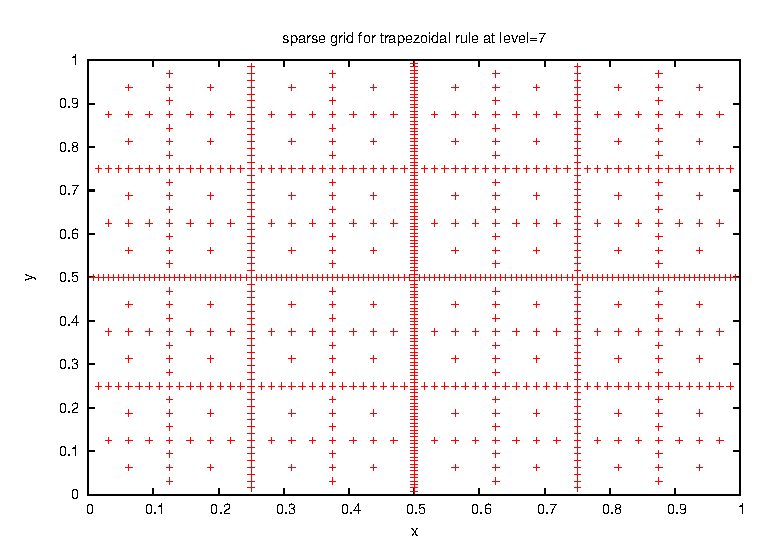
\includegraphics[width=.9\textwidth]{task11_trap_7}
\caption{Trapezoidal sparse grid at level 7}
\label{fig:Task11d}
\end{figure}
\clearpage


\section*{Task 12}
Comparison of product grid and sparse grid.\\
\begin{figure}[!ht]
\centering
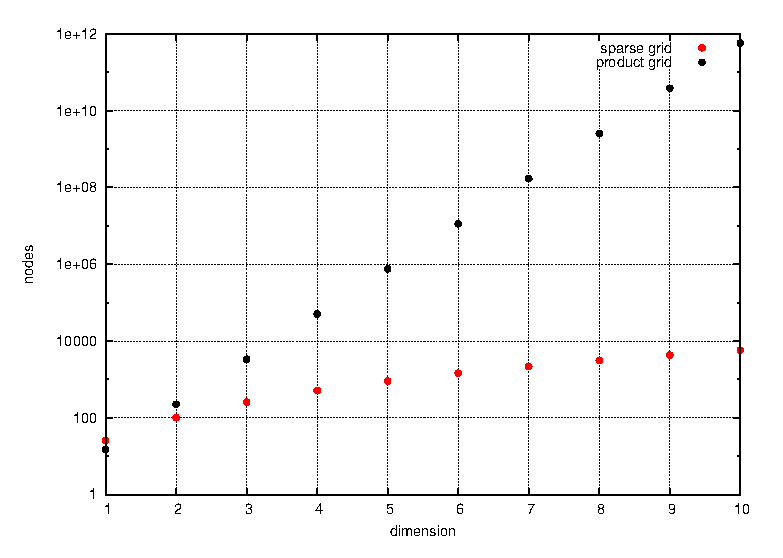
\includegraphics[width=.9\textwidth]{task12}
\caption{Number of points/evaluations for sparse grid/product grid at level 4 for different dimensions}
\label{fig:Task12}
\end{figure}
\clearpage

\section*{Task 13}
Convergence plots for integration of $f(x_1,...,x_d)=\prod_{j=1}^d (1+\gamma\exp(x_j/2)),\gamma=0.1$ for varying dimension $d$ against closed-form solution.\\
\begin{figure}[!ht]
\centering
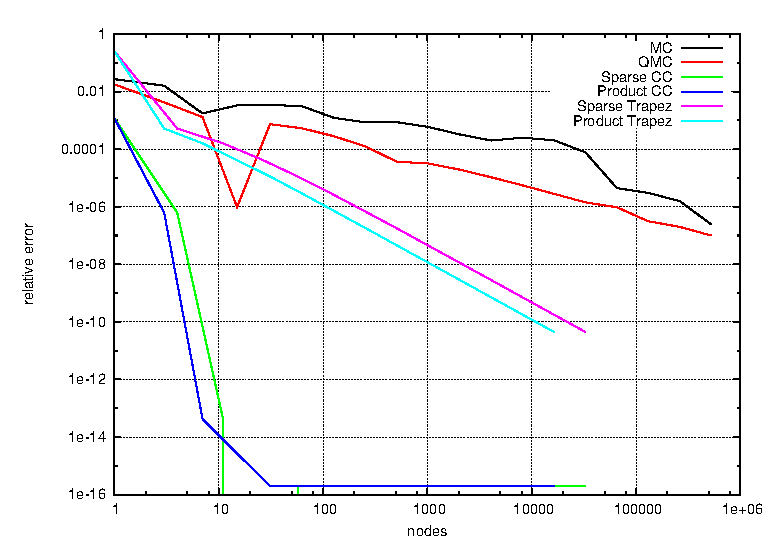
\includegraphics[width=.9\textwidth]{task13_d1}
\caption{Convergence plot for $d=1$}
\label{fig:Task13a}
\end{figure}

\begin{figure}[!ht]
\centering
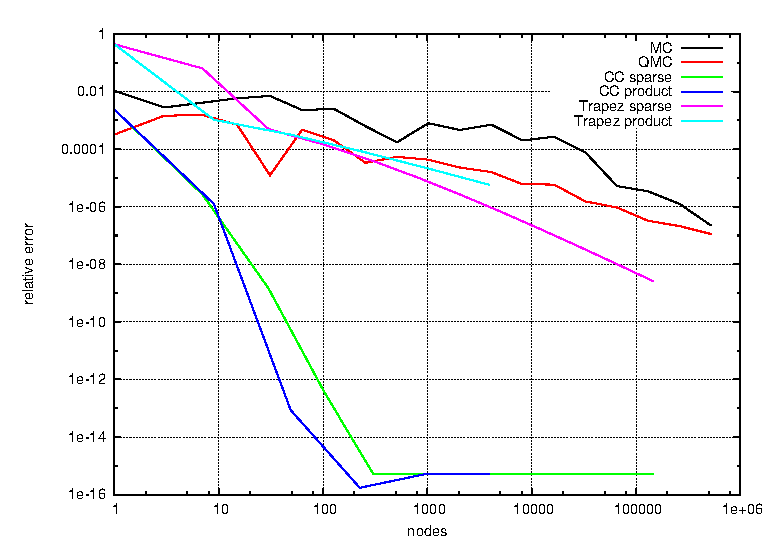
\includegraphics[width=.9\textwidth]{task13_d2}
\caption{Convergence plot for $d=2$}
\label{fig:Task13b}
\end{figure}

\begin{figure}[!ht]
\centering
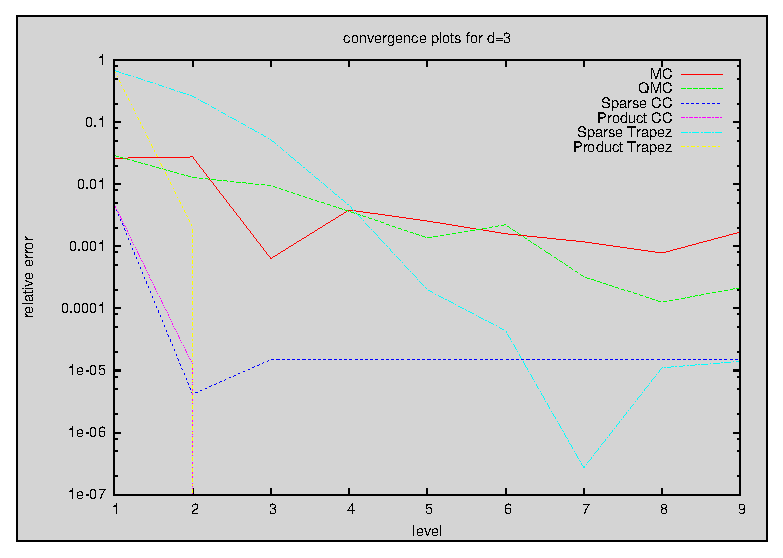
\includegraphics[width=.9\textwidth]{task13_d4}
\caption{Convergence plot for $d=4$}
\label{fig:Task13c}
\end{figure}

\begin{figure}[!ht]
\centering
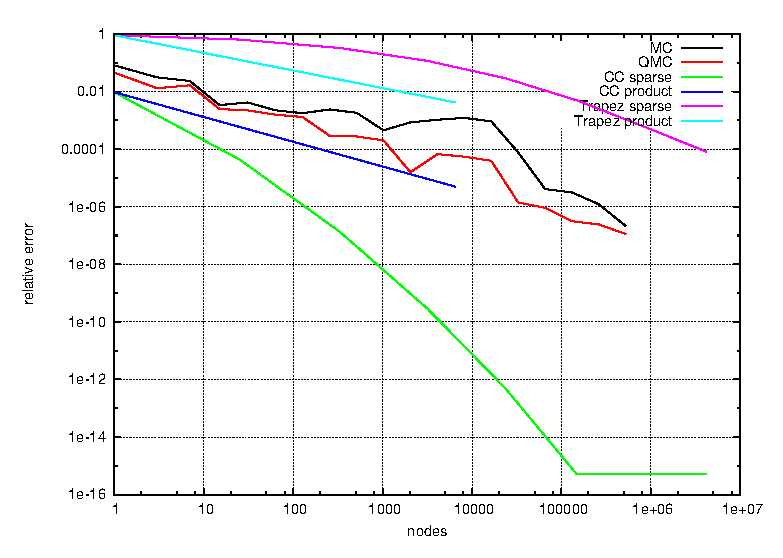
\includegraphics[width=.9\textwidth]{task13_d8}
\caption{Convergence plot for $d=8$}
\label{fig:Task13d}
\end{figure}
\clearpage

\section*{Task 14}
Implementation of Brownian Bridge. See task14.cpp for code.

\section*{Task 15}
Convergence of integration of discrete geometric Asian option with $S(0)=10,r=0.1,\sigma=0.25,T=1,K=0,M=16$ against closed-form solution.
\begin{figure}[!ht]
\centering
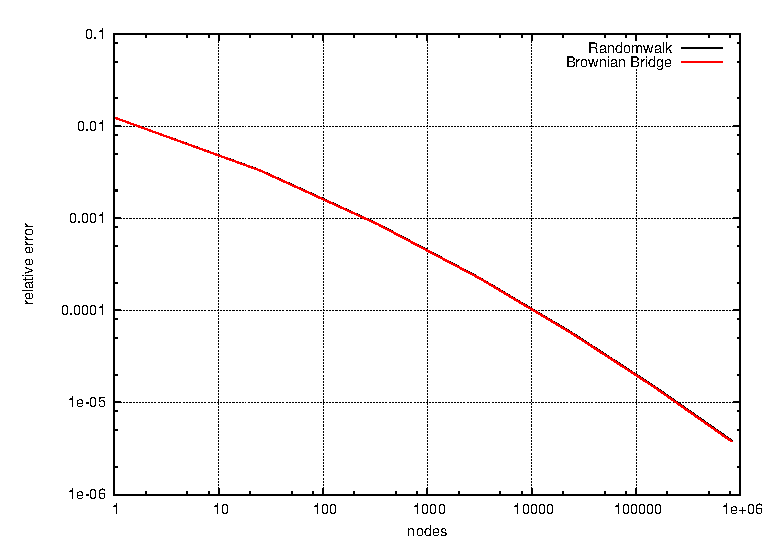
\includegraphics{task15}
\caption{Convergence plot for Clenshaw-Curtis sparse grid}
\label{fig:Task15}
\end{figure}
\clearpage

\section*{Task 16}
Convergence of integration of discrete geometric Asian option with $S(10)=10,r=0.1,\sigma=0.25,T=1,K=0,M=8$ against closed-form solution.

\begin{figure}[!ht]
\centering
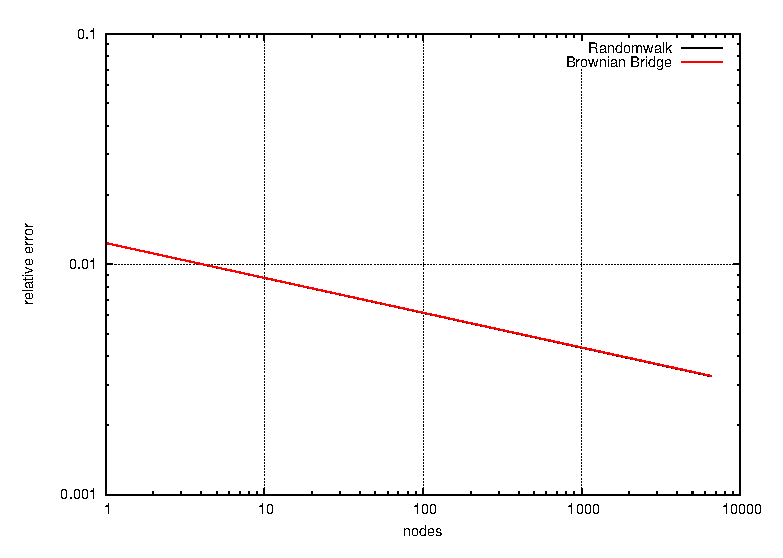
\includegraphics{task16_ccprod}
\caption{Convergence plot for Clenshaw-Curtis product grid}
\label{fig:Task16a}
\end{figure}

\begin{figure}[!ht]
\centering
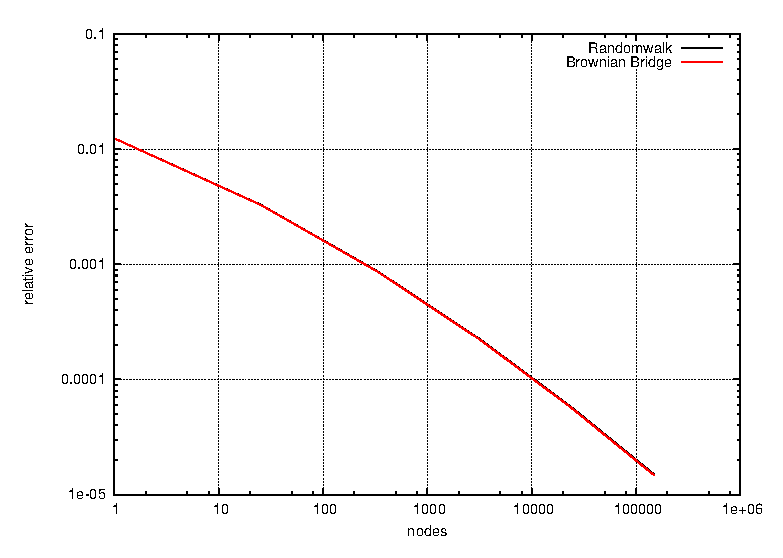
\includegraphics{task16_ccsparse}
\caption{Convergence plot for Clenshaw-Curtis sparse grid}
\label{fig:Task16b}
\end{figure}

\begin{figure}[!ht]
\centering
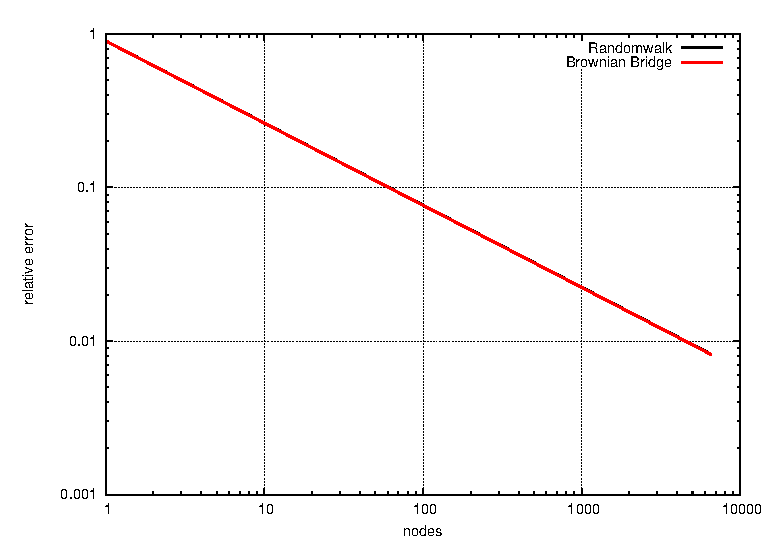
\includegraphics{task16_trapprod}
\caption{Convergence plot for Trapezoidal rule product grid}
\label{fig:Task16c}
\end{figure}

\begin{figure}[!ht]
\centering
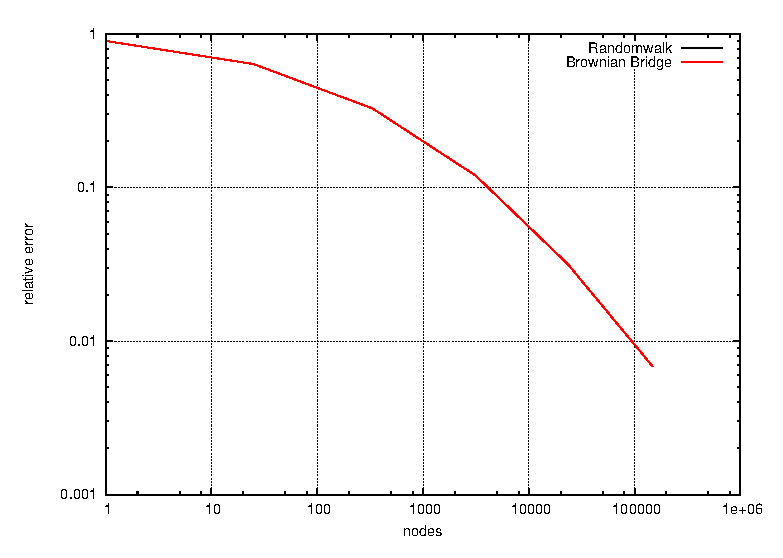
\includegraphics{task16_trapsparse}
\caption{Convergence plot for trapezoidal rule sparse grid }
\label{fig:Task16d}
\end{figure}

\begin{figure}[!ht]
\centering
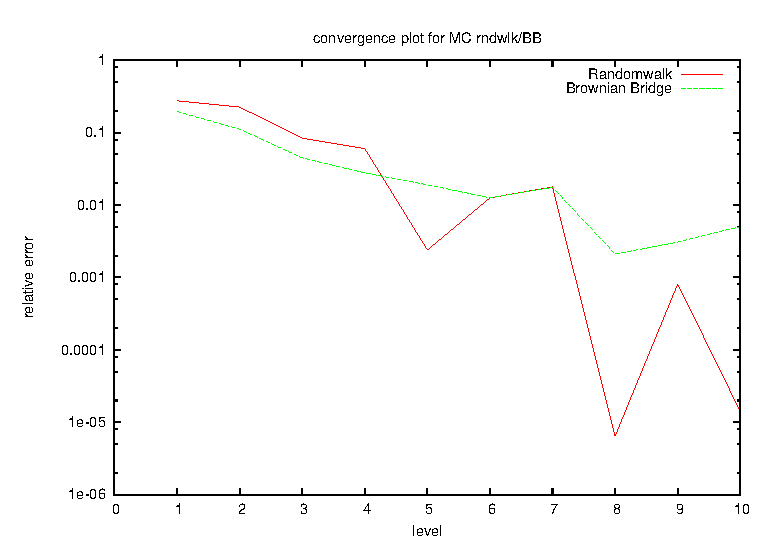
\includegraphics{task16_mc}
\caption{Convergence plot for Monte Carlo}
\label{fig:Task16e}
\end{figure}

\begin{figure}[!ht]
\centering
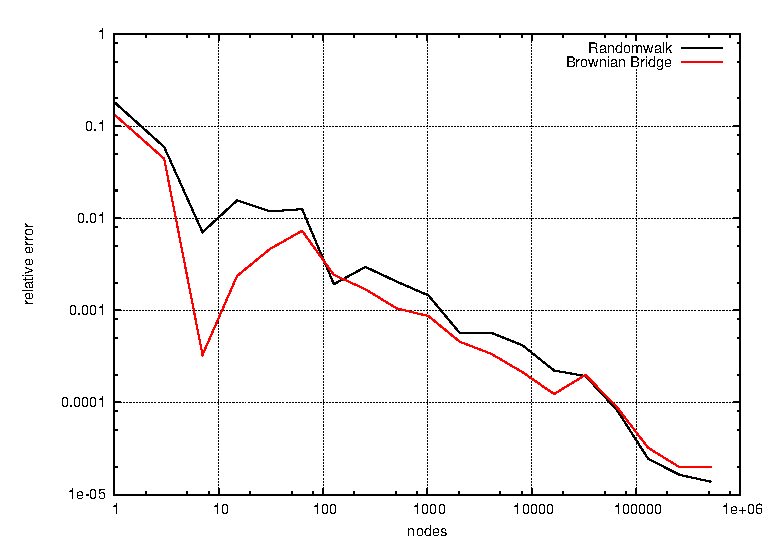
\includegraphics{task16_qmc}
\caption{Convergence plot for Quasi-Monte Carlo}
\label{fig:Task16f}
\end{figure}

\begin{figure}[!ht]
\centering
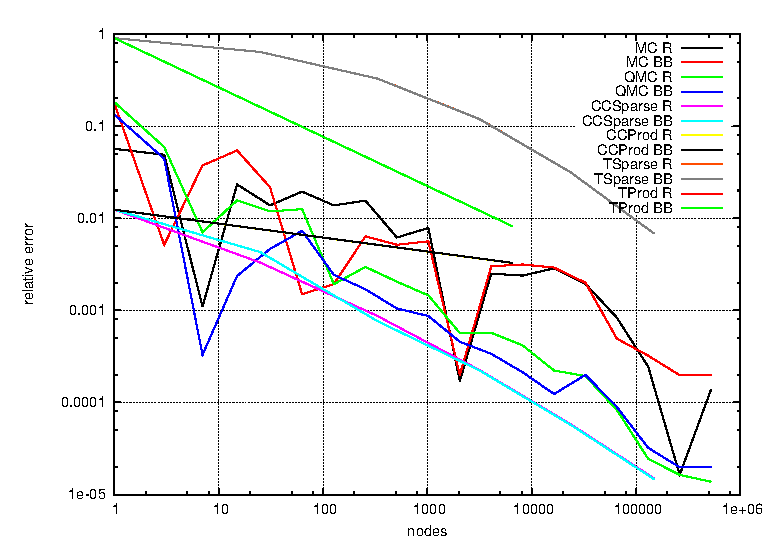
\includegraphics{task16}
\caption{Convergence plot for all methods}
\label{fig:Task16g}
\end{figure}
\clearpage


\section*{Task 17}
Convergence of integration of discrete geometric Asian option with $S(10)=10,r=0.1,\sigma=0.25,T=1,K=10,M=64$ against closed-form solution.
\begin{figure}[!ht]
\centering
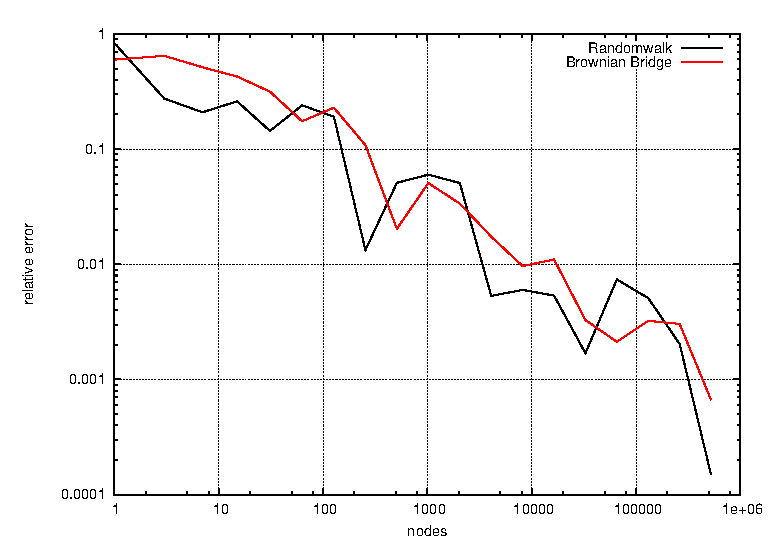
\includegraphics{task17_mc}
\caption{Convergence plot for Monte Carlo}
\label{fig:Task17a}
\end{figure}

\begin{figure}[!ht]
\centering
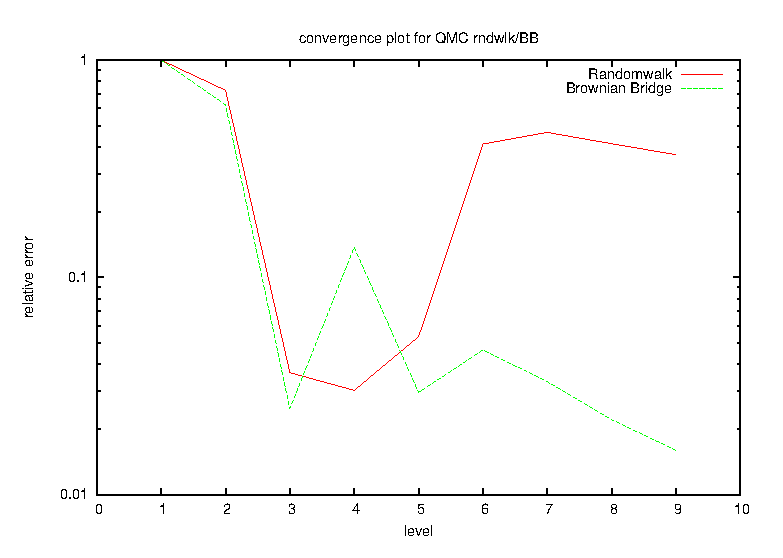
\includegraphics{task17_qmc}
\caption{Convergence plot for Quasi-Monte Carlo}
\label{fig:Task17b}
\end{figure}
\clearpage

\section*{Task 18} It is almost always better to not use (Q)MC, since the other
quadrature rules converge faster (even using full grids) provided the dimension is low and the integrand is continuously differentiable. Clenshaw-Curtis
converges slightly faster than the Trapezoidal rule. In almost all cases sparse
grids are preferrable since they only give us a slightly worse convergence, but
a lot less points of evaluation (see Task 12). But if everything else fails, (Q)MC
works and in high dimensions, MC is better than the other methods (curse of dimension).
\end{document}
